\chapter{Программный комплекс и численные примеры решения задач представленных математических моделей}\label{part4}

В данной главе представлены описание и структура программно-вычислительного комплекса, предназначенного для расчета задачи оптимального размещения БС и результаты численного эксперимента задачи телекоммуникационного покрытия вдоль линейного участка.

\section{Программный комплекс расчета задачи размещения БС}

Программный комплекс \cite{progbib_mukhtarpov} представляет собой реализацию на языке Python алгоритма типа ветвей и границ комбинаторной задачи оптимизации поиска максимального телекоммуникационного покрытия при размещении базовых станций. Код программы представлен в \url{https://github.com/m0000Amir/BST_BS_types_set}.

Структура программно-вычислительного комплекса представлена на рисунке \ref{fig:part4_program_computer}. На вход подается JSON-file, содержащий параметры конфигурации и входные данные задачи.

 Параметы конфигурации расположены под ключом $\textbf{configuration}$ (Рисунок \cref{fig:part4_input_data_configuration}):
 \begin{itemize}
   \item $\textbf{method}$ -- метод решения задачи размещения. Значение $\textit{bab}$ -- метод ветвей и границ или $\textit{bf}$  -- метод полного перебора;
   \item $\textbf{estimation\_method}$ -- метод расчета оценки недопокрытия справа. Значение $\textit{LP}$ -- решение с помощью сиплекс-метода, значение $\textit{ILP}$ -- решение с помощью задача целочисленного линейного программирования или значение $\textit{knapsack}$ -- решение с помощью задачи <<О ранце>>;
   \item $\textbf{placed\_all\_station}$ -- частный случай задачи размещения, когда отсутствуют ограничения на стоимость и времени задержки, в такой постановек размещается все множество станций. Принимает значения $\textit{True}$ или $\textit{False}$;
   \item $\textbf{drawing}$ -- отрисовка полученного дерева решения.  Принимает значения $\textit{True}$ или $\textit{False}$;
   \item $\textbf{last\_optimal\_noncoverage}$ -- полученное оптимальное недопокрытия на последнем решении  для задачи поиска последовательности лучших решений. Принимает любые положительные действительные значения;
   \item $\textbf{relation\_deviation}$ -- заданное отклонение в процентах от полученного оптимального решения для задачи поиска последовательности лучших решений.
 \end{itemize}



\begin{figure}[h!]
  \centering
   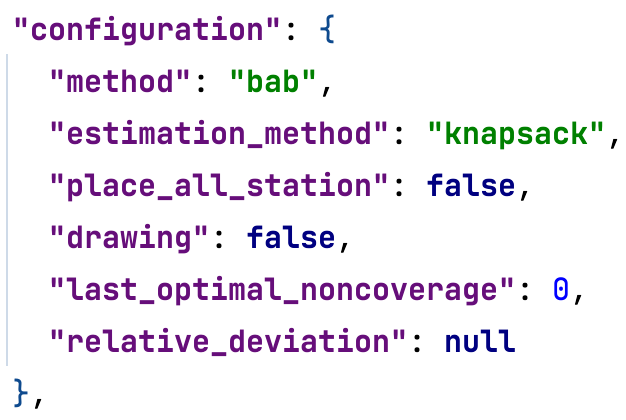
\includegraphics[width=.5\textwidth]{input_data_configuration.png}
\caption{Параметры конфигурации}
\label{fig:part4_input_data_configuration}
\end{figure}

Файл JSON содержит входные данные задачи оптимизации: 
\begin{itemize}
  \item координаты размещения $\textbf{placement}$ и координаты размещения шлюзов $\textbf{gateway\_placement}$;
  \item  параметры антенн шлюзов $\textbf{gateway}$ и абонентских устройств $\textbf{user\_device}$;
  \item ограничения задачи на стоимость $\textbf{cost\_limit}$ и время задержки $\textbf{delay\_limit}$;
  \item параметры для расчета дальности телекоммуникационного покрытия: несущая частота $\textbf{frequency}$, запас на замирания сигнала $\textbf{link\_som}$ и $\textbf{coverage\_som}$;
  \item параметры для расчета задержек: средний размер пакетов $\textbf{average\_packet\_size}$ и интенсивность входящего потока $\textbf{arrival\_rate}$;
  \item $\textbf{sta}$ -- множество заданных базовых станций.
\end{itemize}

\begin{figure}[h!]
  \centering
   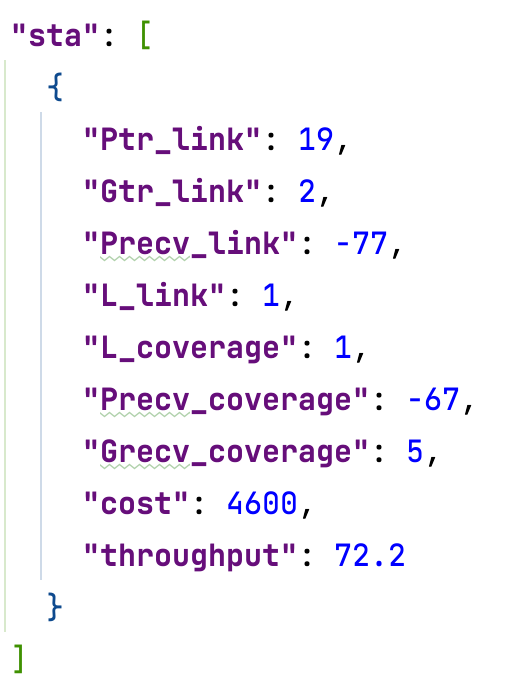
\includegraphics[width=.4\textwidth]{input_data_sta.png}
\caption{Параметры БС}
\label{fig:part4_input_data_sta}
\end{figure}

Каждый элемент массива $\textbf{sta}$ (Рисунок \cref{fig:part4_input_data_sta}) представляет собой JSON-объект и содержит следующие параметры:
\begin{itemize}
  \item $\textbf{Ptr\_link}$ -- мощность антенны, обеспечивающей телекоммуникационную связь между станциями;
  \item $\textbf{Gtr\_link}$ -- усиления антенны, обеспечивающей телекоммуникационную связь между станциями;
  \item $\textbf{Precv\_link}$ -- чувствительность антенны, обеспечивающей телекоммуникационную связь между станциями;
  \item $\textbf{L\_link}$ -- потери сигнала в кабеле и разъемах передающего тракта антенны, обеспечивающей телекоммуникационную связь между станциями;
  \item $\textbf{L\_coverage}$ -- потери сигнала в кабеле и разъемах передающего тракта антенны, обеспечивающей телекоммуникационное покрытие БС;
  \item $\textbf{Precv\_coverage}$ -- чувствительность антенны, обеспечивающей телекоммуникационное покрытие БС;
  \item $\textbf{Grecv\_coverage}$ -- усиления антенны, обеспечивающей телекоммуникационное покрытие БС;
  \item $\textbf{cost}$ -- стоимость БС;
  \item $\textbf{throughput}$ -- пропускная способность БС.
\end{itemize}



\begin{figure}[h!]
  \centering
   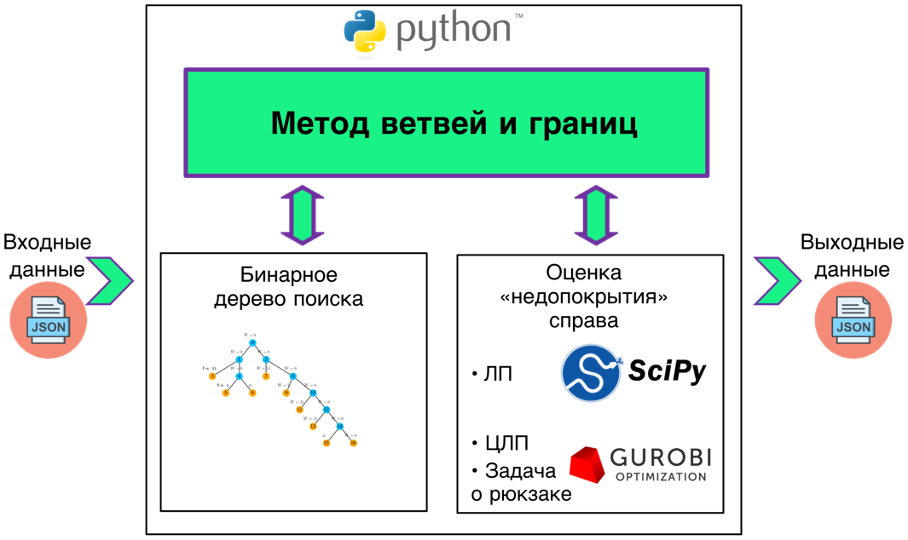
\includegraphics[width=.95\textwidth]{program_computer.png}
\caption{Cтруктура программно-вычислительного комплекса}
\label{fig:part4_program_computer}
\end{figure}

Перед тем как приступить к задаче размещения, необходимо подготовить параметры для каждой станции: радиус связи между станциями и радиус покрытия БС. Параметры рассчитываются в блоке расчета дальности телекоммуникационной связи с помощью уравнения энергетического потенциала линии связи и моделей распространения сигнала. Модели распространения представлены в главе 1.


Задача размещения базовых станций представлена в виде комбинаторной модели в экстремальной форме. Алгоритм поиска оптимального размещения относится к типу ветвей и границ. 

Для поиска оптимального размещения используется процедура построения бинарного дерева поиска. На каждом шаге проверяется условия на возможность закрытие узла дерева. Построение бинарного дерева поиска реализовано рекуррентным способом.

Блок оценки недопокрытия справа представляет собой три варианта расчета. \underline{\textit{\textbf{Задача 2}}} представляет собой задачу ЦЛП, \underline{\textit{\textbf{задача 3}}} является задачей <<О ранце>>. \underline{\textit{\textbf{Задача 4}}} представляет собой задачу ЛП. Задача ЦЛП и задача <<О ранце>> рассчитывается в коммерческом продукте расчета задач дискретной оптимизации Gurobi Optimizer \cite{gurobi}. Задача ЛП решается с использованием библиотеки для языка программирования Python с открытым исходным кодом SciPy \cite{scipy}. 


\begin{figure}[h!]
  \centering
   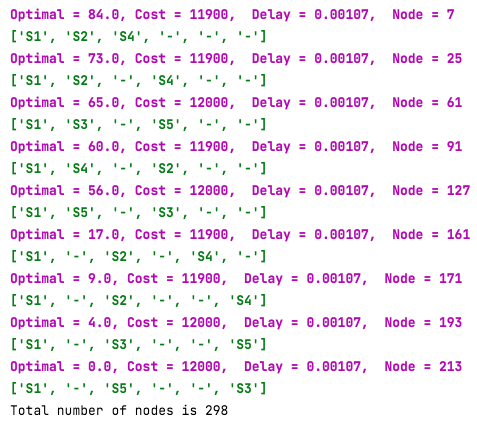
\includegraphics[width=.6\textwidth]{problem_output.png}
\caption{Пример полученного решения задачи}
\label{fig:part4_problem_output}
\end{figure}

В ходе движения по дереву поиска записываются все полученные рекорды \textbf{Optimal} (Рисунок \cref{fig:part4_problem_output}). Также записываются стоимость размещения \textbf{Cost}, время межконцевой задержки \textbf{Delay} и номер узла дерева \textbf{Node}, на котором был получен рекорд. Для каждого рекорда записывается множество размещенных станций. Последний полученный рекорд является оптимальным решением задачи. Решение задачи записывается в выходной JSON-файл.

% Алгоритм на основе метода ветвей и границ основан на следующих построениях, позволяющих уменьшить время перебора:


% \begin{enumerate}
%   \item Ветвление. Разбиение исходного множества на попарно не пересекающие дочерние подмножества в ходе поиска оптимального решения.
%   \item Получение нижних границ. Исследования текущей вершины на возможность закрытия.
% \end{enumerate}

% Особенность задачи дискретного программирования состоит в том, что они имеют переборный характер. Основная идея комбинаторных алгоритмов -- выделить из множества допустимых решений подмножества, не содержащие оптимальных решений \cite{SigalBook}, для сокращения времени перебора всех возможных вариантов. 


% Опишем процедуру построения бинарного дерева поиска (дерева ветвлений) для полного перебора без повторений всех элементов множества $\Gamma$. Данная процедура будет использована при построении дерева поиска в алгоритме МВиГ решения \textbf{задачи 1}.

% Предполагается, что в множестве $S$ станции упорядочены по не убыванию радиусов покрытия. Описываемая процедура использует известный прием разбиения множества $G$ на подмножества с использованием некоторого параметра. Процесс формирования и последовательность исследования подмножеств обычно представляется с помощью дерева поиска, представляющего собой ориентированное от корня «дерева ветвлений», где каждому подмножеству соответствует вершина на дереве. Множеству $\Gamma$ соответствует корневая вершина. 

\FloatBarrier
\section{Численный пример оптимального размещения базовых станций сети с линейной топологией в виде задачи целочисленного линейного программирования}\label{part4:ilp_solution}

Рассмотрим пример задачи оптимального размещения БС вдоль линейного участка для организации БШС на базе семейства протоколов IEEE 802.11. Задан линейный участок $L =230$ метров. На данном участке были отобраны $|A| =6$ возможных точек размещения базовых станций с координатами $l_i$, представленными в таблице \cref{tab:placement_point_mip}. Задано множество станций $|S| =5$. Задано бюджетное ограничение $C = 12000$ руб. На концах участка размещены шлюзы $s_0 $ и $s_{m+1}$ с параметрами (таблица \cref{tab:part4_gateway_parameters_mip})

\begin{table}[h!]\centering
  \begin{tabular}{|c||c|c|c|c|c|c|}\hline
      Точки размещения, $a_i$ &	$a_1$&	$a_2$&	$a_3$&	$a_4$&	$a_5$&	$a_6$ \\
      \hline
      Координаты, $l_i$ &	36&	51&	115&	135&	182&	191\\
      \hline
\end{tabular}\caption{Координаты точек размещения}\label{tab:placement_point_mip}
\end{table}


\begin{table}[h!]\centering
  \begin{tabular}{|c||c|c|c|c|}\hline
      
      Шлюз&	$P_{tr}^R$&	$P_{recv}^R$& $G_{recv}^R$&	$L$ \\
      \hline
      \textnumero&	дБ&	дБ&	дБ&	дБ \\
      \hline
      $s_0 $& 20&	-77&	5& 1 \\
      $s_{m+1}$& 20& -77&	5& 	1 \\
      \hline

\end{tabular}\caption{Параметры шлюзов}\label{tab:part4_gateway_parameters_mip}
\end{table}

Требуется найти максимальное телекоммуникационного покрытия заданного участка с учетом ограничением на стоимость и условием обеспечения связи между заданными шлюзами через систему размещенных БС.


На рынке представлен широкий спектр технических устройств от компаний Cisco, Mikrotik и т.д., позволяющих организовывать сеть в открытой местности и учитывающие климатические сложности, как например на нефтегазовых месторождениях, такие как предельные температуры, сила ветра и т.д. Под БС  будем понимать точку доступа с антеннами для обеспечения телекоммуникационного покрытия заданной области и антеннами для обеспечения телекоммуникационной связи с соседними станциями БШС. 

В ходе этапа выбора комплекса технических средств были отобраны $|S| = 5$ БС. Каждой БС приписаны паспортные характеристики антенн и итоговая стоимость станции. Стоимость взята условная, чтобы не указывать реальные цены производителя на время написания диссертации и курс валют. Рабочая частота 2,4 ГГц. В таблице \cref{tab:part4_sta_parameters_mip} представлены параметры БС. Верхний индекс $R$ указывает на характеристики антенн для связи между станциями, верхний индекс $r$ указывает на характеристики антенн для покрытия заданного участка. Здесь $P_{tr}^{R}$ -- мощность направленной антенны, $G_{tr}^R$ -- усиление направленной антенны, $P_{recv}^R$ -- чувствительность направленной антенны, $L$  -- потери в антенном кабеле и разъемах, передающего тракта, $P_{recv}^r$ -- чувствительность всенаправленной антенны, $G_{recv}^r$ -- усиление всенаправленной антенны и $c$ – стоимость.

\begin{table}[h!]\centering
  \begin{tabular}{|c||c|c|c|c|c|c|c|}\hline
      
      S&	$P_{tr}^R$&	$G_{tr}^R$&	$P_{recv}^R$&	$L$&	$P_{recv}^r$&	$G_{recv}^r$&		$c$ \\
      \hline
      &	дБм&	дБ&	дБм&	дБ&	дБм&	дБ&		руб. \\
      \hline
      1&	19&	2&	-77&	1&	-67&	5&	  4600 \\
      2&	20&	2&	-77&	1&	-73&	2&		4100 \\
      3&	19&	2&	-77&	1&	-73&	2&		3800 \\
      4&	19&	2&	-75&	1&	-70&	2&		3200 \\
      5&	18&	2&	-77&	1&	-67&	4&		3600 \\
      \hline
  \end{tabular}\caption{Параметры БС для задачи ЦЛП}\label{tab:part4_sta_parameters_mip}
\end{table}


Для расчета области покрытия необходимо задаться характеристиками пользовательских устройств, с которых будет собираться информация (таблица \cref{tab:part4_user_device_parameters_mip}).


\begin{table}[h!]\centering
  \begin{tabular}{|c||c|c|c|}\hline    
    \multirow{2}{*}{Устройство}&	$P_{tr}^{ud}$&	$G_{tr}^{ud}$&	$L^{ud}$ \\ \cline{2-4}
    &	дБ&	дБ&	дБ	 \\ \cline{2-4}
    % \hline
    &	9&	1&	0 \\
    \hline
  \end{tabular}\caption{Параметры устройств}\label{tab:part4_user_device_parameters_mip}
\end{table}



% \fixme{Переделать численный пример}
% В этой секции представлен численный пример решения данной задачи.
% % This section shows one simple case of the problem.

% Задан линейный участок $L$ с длиной 300 с количеством $n=7$ точек размещения. Координаты точек размещения представлены в таблице \cref{tab:part3_placed_point}.  Задан бюджет размещения $C=130$. Центральная частота $f = 2437$ МГц. 

% \begin{table}[h!]\centering
%   \begin{tabular}{|c||c|c|c|c|c|c|c|}\hline
%     $a_i$ & $a_1$ &  $a_2$ & $a_3$ & $a_4$ & $a_5$ & $a_6$ & $a_7$ \\ \hline \hline
%     Координата & 29 & 40 & 95 & 139 & 181 & 230 & 273 \\ \hline
% \end{tabular}\caption{Точки размещения участка с длиной $L = 300$.}\label{tab:part3_placed_point}
% \end{table}

% % Задано множества базовых станций $m = 8$ с параметрами представленными в таблице \cref{tab:part3_BS}. Также в таблице представлены параметры шлюзов и контролируемых объектов. Параметры объектов необходимы для расчета радиусов покрытия станций.

% \begin{table}[b]\centering
%   \begin{tabular}{|c||c|c|c|c|c|c|c|}\hline
%     BS & $P_{tr}^R$ &  $G_{tr}^R$ & $P_{recv}^R$ & $P_{recv}^r$ & $G_{recv}^r$ & $c$ \\ \cline{2-1} \cline{3-1} \cline{4-1} \cline{5-1}  \cline{6-1} \cline{7-1}
%      & дБм & дБ & Дбм & дБм & дБ & у.е.  \\ \hline
%     1 & 20 & 5 & -69 & -67 & 5 & 40 \\ 

%     2 & 19 & 5 & -67 & -67 & 5 & 28 \\ 

%     3 & 18 & 5 & -69 & -67 & 5 & 45 \\ 

%     4 & 19 & 5 & -69 & -67 & 6 & 22 \\ 

%     5 & 19 & 5 & -67 & -67 & 5 & 21 \\ 

%     6 & 20 & 5 & -69 & -67 & 5 & 40 \\ 

%     7 & 19 & 5 & -67 & -67 & 5 & 28 \\

%     8 & 18 & 5 & -69 & -67 & 5 & 45 \\ \hline \hline  

%     &  $G_{recv}^R$ & $P_{recv}^R$ &  & & $P_{tr}^r$ & $G_{tr}^r$ \\  \cline{2-1} \cline{3-1} \cline{6-1} \cline{7-1} 

%     Шлюз& дБ & дБм & & Объект & дБм & дБ  \\  \cline{2-1} \cline{3-1}  \cline{6-1} \cline{7-1}

%     &  5 & -69 & &  & 15 & 2  \\ \hline

%   \end{tabular}\caption{Параметры базовых станций, шлюзов и объектов.}\label{tab:part3_BS} 
% \end{table}

Необходим подготовить параметры станций: радиус связи$R_{jq}$ и радиус покрытия $r_j$. В обоих случаях воспользуемся уравнение потерь в свободном пространстве. Для расчета связи между станциями запас на замирания сигнала ($SOM$) примем равным 20 дБ и для расчета области покрытия равным 14 дБ.

\textbf{Расчет радиуса связи между станциями.}
% Базовые станции оснащены направленной антенной с высоким коэффициентом усиления для связи с соседними станциями.
Расчет потерь между станциями $s_j$ и $s_q$, согласно формуле \cref{eq:part3_L_fs_from_link_budget} выражается как


\begin{displaymath}
  L_{fs}^{jq} = P_{tr}^R(j) - L(j) + G_{tr}^R(j) + G_{tr}^R(q) - L(q) - P_{recv}^R(q) - SOM.
\end{displaymath}


Для примера представлен расчет радиуса связи между станциями $s_1 $ и $ s_2 $:

\begin{align}
  \begin{aligned}
  L_{fs}^{12} = P_{tr}^R(1) - L(1) + G_{tr}^R(1) + G_{tr}^R(2) - L(2) - P_{recv}^R(2) - SOM = \\
  = 19 - 1 + 2 + 2 - 1 - (-69) - 20  = 78 (\text{дБ}).
  \end{aligned}
\end{align}

Для расчета дальности связи воспользуемся формулой \cref{eq:part1_fspl_model_r}. Несущая частота $ F = 2437 $ МГц и коэффициент для расчета потерь $ K = -27,55 $:

% \fixme{Формула не верна расчета $R_{jq}$}

\begin{align}
  \begin{aligned}
  R_{jq} = 10^{\left(\frac{L_{fs}^{jq} - 20\lg{F} + G_{tr}^R(j) + G_{tr}^R(q) - K}{20}\right)}
  = \\ 10^{\left(\frac{78 - 20\lg{2437} + 2 + 2 - (-27.55)}{20}\right)} = 123 (\text{м}).
  \end{aligned}
\end{align}

В таблице \cref{tab:part4_Rjq_mip} приведены радиусы связи между всеми станциями $ s_j $, $ j = 1, ..., m $ и шлюзом $ s_ {m + 1} $.

\begin{table}[h!]\centering
  \begin{tabular}{|c||c|c|c|c|c|c|c|}\hline
      $R_{jq}$ & $s_1$ & $s_2$ & $s_3$ & $s_4$ & $s_5$ & $s_{0}$ & $s_{m+1}$ \\ \hline \hline

      $s_1$ &--& 123& 123& 98& 123& 246& 246\\ 
      $s_2$ &138& --& 138& 110& 138& 276& 276\\ 
      $s_3$ &123& 123& --& 98& 123& 246& 246\\ 
      $s_4$ &123& 123& 123& --& 123& 246& 246\\ 
      $s_5$ &195& 155& 195& 195& --& 276& 219\\ 
      $s_{0}$ &276& 276& 276& 219& 276& --& --\\
      $s_{m+1}$ &276& 276& 276& 219& 276& --& --\\  
      \hline

\end{tabular}\caption{Рассчитанные радиусы связи между станциями}\label{tab:part4_Rjq_mip}
\end{table}

\textbf{Расчет радиуса покрытия}

% Для покрытия заданного участка базовая станция оснащена всенаправленной антенной с выходной мощностью $ P_{tr}^r $ и усилением $ G_{tr}^r$. Потери в кабеле $ L_ {tr} $ равно 1.

% To cover a given section, the base station is equipped with an isotropic antenna with output power $ P_ {tr} ^ r $ and gain $ G_ {tr} ^ r $ is equal to 0. The cable loss $ L_ {tr} $ is equal to 1.

% A coverage area depends on a base station, as well as user device characteristics. Let us consider a user device with an antenna sensitivity $P_{RX} = -67$ dBm and gain $G_{RX} = 0$. Loss $L_{RX}$ is equal to 0.
Расчет проводится аналогично расчета радиусу связи между станциями. 
Потери в свободном пространстве для канала между $j$-ой станции и контролируемым объектом

\begin{displaymath}
  % L_{fs}^{j} = P_{tr}^r(j) - L_{tr}  - SOM - P_{RX}.
  L_{fs}^{j} = P_{tr}^{ud} - L^{ud} + G_{tr}^{ud} + G_{recv}^r(j) - L(j) - P_{recv}^r(j) - SOM.
\end{displaymath}


Пример расчета радиуса покрытия для станции $s_1$:

\begin{align}
    \begin{aligned}
  % L_{fs}^{1} = P_{tr}^r + G_{tr}^r + G_{recv}^r(1) - L_{recv}(1)  - SOM - P_{recv}^r(1) = \\
%  = 15+2+5-1-(-67)-10 = 78 \text{ (дБ)}.
 L_{fs}^{1} = P_{tr}^{ud} - L^{ud} + G_{tr}^{ud} + G_{recv}^r(1) - L(1) - P_{recv}^r(1) - SOM = \\ = 9 - 0 + 1 + 5 - 1 - (-67) - 14 = 67 \text{ (дБ)}.
    \end{aligned}
\end{align}

\begin{displaymath}
  r_{1} = 10^{\left(\frac{67 - 20\lg{2437} + 1 + 5 - (-27.55)}{20}\right)} = 44 \text{ (м)}.
\end{displaymath}

Радиусы покрытия для всех станций $ s_j $, $ j = \overline{1, m} $ представлены в таблице \cref{tab:part4_rj_mip}).

\begin{table}[h!]\begin{center}
  \begin{tabular}{|c||c|c|c|c|c|c|c|c|}\hline
      STA & $s_1$ & $s_2$ & $s_3$ & $s_4$ & $s_5$ & $s_{0}$ & $s_{m+1}$\\ \hline \hline
      $r_{j}$ & 44 & 44 & 44 & 31 & 35 & 0 & 0\\ \hline
\end{tabular}\caption{Рассчитанные радиусы покрытия станций}\label{tab:part4_rj_mip}
\end{center}
\end{table}

Теперь можно приступить к решению задачи ЦЛП. Математическая модель задачи ЦЛП \cref{eq:part3_objective_function} -- \cref{eq:part3_cost} написана в коммерческом продукте Matlab и решена с Optimization Toolbox \cite{optimization_toolbox}. Код программы представлен в \url{https://github.com/m0000Amir/ILP}.
 

% Задача ЦЛП решена с помощью Optimization Toolbox MatLab. Таблица \cref{tab:part4_ilp_solution} содержит все полученные целочисленные решения.


\begin{table}[h!]\tiny\centering
  \begin{tabular}{|c||c|c|c|c|c|c||c|c|}\hline
    $a_i$ & $a_1$ &  $a_2$ & $a_3$ & $a_4$ & $a_5$ & $a_6$   & Покрытие & Цена \\ \hline 
    Координаты & 36 & 51 & 115 & 135 & 182 & 191 & м & руб.\\ \hline \hline
    Целочисленное решение 1 & --  & $s_2$ & $s_3$ & -- & -- & $s_5$ & 219 & 11500\\ 
    Целочисленное решение 2 & $s_5$ & -- & $s_1$ & -- & -- & $s_3$ & 229 & 12000\\
    Оптимальное решение & $s_2$ & -- & $s_5$ & -- & -- & $s_3$ & 230 & 11500 \\ \hline
\end{tabular}\caption{Решение задачи ЦЛП}\label{tab:part4_ilp_solution}
\end{table}

В ходе движения по дереву поиска было получено 3 целочисленных решения. Оптимальным решением является последнее найденное целочисленное решения. Результаты решения представлены в таблице \cref{tab:part4_ilp_solution}. Величина покрытия полученного размещения равна 230 метров, суммарная стоимость составила 11500 руб.


% \fixme{=================================================}

\FloatBarrier
\section{Численный пример оптимального размещения базовых станций сети с линейной топологией в виде экстремальной задачи в комбинаторной форме}\label{part4:bnb_solution}

Теперь решим эту же задачу с помощью предложенного алгоритма. Кроме бюджетного ограничения, будем учитывать ограничение на время задержки в БШС. Предложенный алгоритм позволяет получить не только оптимальное размещение, но и последовательность лучших размещений. При проектировании БШС такой подход позволяет проверить допустимые решения, когда оптимальное решение не удовлетворяет требования на следующих этапах после синтеза топологии БШС.

% Рассмотрим пример задачи оптимального размещения БС вдоль линейного участка для организации БШС на базе семейства протоколов IEEE 802.11.

Задан линейный участок $L =230$ метров, на котором необходимо разместить БС для организации БШС на базе семейства протоколов IEEE 802.11. Заданы $|A| =6$ возможных точек размещения базовых станций с координатами $l_i$ (таблица \cref{tab:placement_point_mip}). Задано множество станций $|S| =5$. Задано бюджетное ограничение $C = 12000$ руб. и ограничение на время доставки пакетов $T = 0,5$  мс. Будем считать, что на каждую БС пакеты поступают со средним размером пакетов $w = 1500$ байт (0,012 Мбит) и с интенсивностью $\lambda = 100$ $c^{-1}$. Для поиска допустимых размещений задано отклонение от оптимального $\varepsilon = 0,5 \%$.

% \begin{table}[h!]\centering
%   \begin{tabular}{|c||c|c|c|c|c|c|}\hline
%       Точки размещения, $a_i$ &	$a_1$&	$a_2$&	$a_3$&	$a_4$&	$a_5$&	$a_6$ \\
%       \hline
%       Координаты, $l_i$ &	36&	51&	115&	135&	182&	191\\
%       \hline
% \end{tabular}\caption{Координаты точек размещения для комбинаторной модели}\label{tab:placement_point}
% \end{table}

На концах участка размещены шлюзы $s_0 $ и $s_{m+1}$ с параметрами в таблице \cref{tab:part4_gateway_parameters_mip}. Характеристиками пользовательских устройств представлены в таблице \cref{tab:part4_user_device_parameters_mip}.

% \begin{table}[h!]\centering
%   \begin{tabular}{|c||c|c|c|c|}\hline
      
%       Шлюз&	$P_{tr}^R$&	$P_{recv}^R$& $G_{recv}^R$&	$L$ \\
%       \hline
%       №&	дБ&	дБ&	дБ&	дБ \\
%       \hline
%       $s_0 $&	-77&	5& 1 \\
%       $s_{m+1}$& -77&	5& 	1 \\
%       \hline

% \end{tabular}\caption{Параметры шлюзов}\label{tab:part4_gateway_parameters}
% \end{table}

Требуется найти максимальное телекоммуникационного покрытия заданного участка с учетом ограничением на стоимость и время задержки пакетов и условием обеспечения связи между заданными шлюзами через систему размещенных БС.


% На рынке представлен широкий спектр технических устройств от компаний Cisco, Mikrotik и т.д., позволяющих организовывать сеть в открытой местности и учитывающие климатические сложности, например на нефтегазовых месторождениях, такие как предельные температуры, сила ветра и т.д. Под БС  будем понимать точку доступа с антеннами для покрытия заданной области и антеннами для обеспечения связи с соседними станциями БШС. 

В ходе этапа выбора комплекса технических средств были отобраны $|S| = 5$ БС. Каждой БС приписаны паспортные характеристики антенн, пропускная способность точки доступа и итоговая стоимость станции.  Будем рассматривать БШС для задачи мониторинга, то есть с каналом передачи на верхний уровень, UL. Рабочая частота 2,4 ГГц. Для каждой БС будем использовать пропускную способность для модуляции и схемы кодирования MCS7.  В таблице \cref{tab:sta_parameters_bnb} представлены параметры БС. Верхний индекс $R$ указывает на характеристики антенн для связи между станциями, верхний индекс $r$ указывает на характеристики антенн для покрытия заданного участка. Здесь $P_{tr}^{R}$ -- мощность направленной антенны, $G_{tr}^R$ -- усиление направленной антенны, $P_{recv}^R$ -- чувствительность направленной антенны, $L$  -- потери в антенном кабеле и разъемах, передающего тракта, $P_{recv}^r$ -- чувствительность всенаправленной антенны, $G_{recv}^r$ -- усиление всенаправленной антенны,  $p$ – пропускная способность, $c$ – стоимость.

\begin{table}[h!]\centering
  \begin{tabular}{|c||c|c|c|c|c|c|c|c|}\hline
      
      S&	$P_{tr}^R$&	$G_{tr}^R$&	$P_{recv}^R$&	$L$&	$P_{recv}^r$&	$G_{recv}^r$&	$p$&	$c$ \\
      \hline
      \textnumero&	дБм&	дБ&	дБм&	дБ&	дБм&	дБ&	Мбит/с&	руб. \\
      \hline
      1&	19&	2&	-77&	1&	-67&	5&	72,2& 4600 \\
      2&	20&	2&	-77&	1&	-73&	2&	72,2&	4100 \\
      3&	19&	2&	-77&	1&	-73&	2&	72,2&	3800 \\
      4&	19&	2&	-75&	1&	-70&	2&	72,2&	3200 \\
      5&	18&	2&	-77&	1&	-67&	4&	72,2&	3600 \\
      \hline
  \end{tabular}\caption{Параметры БС для задачи в комбинаторной форме}\label{tab:sta_parameters_bnb}
\end{table}


% Для расчета области покрытия необходимо задаться характеристиками пользовательских устройств, с которых будет собираться информация (таблица \cref{tab:part4_user_device_parameters}).


% \begin{table}[h!]\centering
%   \begin{tabular}{|c||c|c|c|}\hline    
%     \multirow{2}{*}{Устройство}&	$P_{tr}^ud$&	$G_{tr}^ud$&	$L$ \\ \cline{2-4}
%     &	дБ&	дБ&	дБ	 \\ \cline{2-4}
%     % \hline
%     &	9&	1&	0 \\
%     \hline
%   \end{tabular}\caption{Параметры устройств}\label{tab:part4_user_device_parameters}
% \end{table}


% Итоговое размещение БС должно удовлетворять заданным ограничениям:
% \begin{itemize}
%   \item на стоимость $C = 76$;
%   \item на межконцевую задержку сети $T =0.001$ с.
% \end{itemize}
% Для расчета времени межкоцневой задержки, будем считать, что на каждую БС поступает трафик с интенсивностью $\lambda = 1000$ 1/с. Средний размер поступающих пакетов $w=1500$ байт.

% Для поиска последовательности топологий задано отклонение $\varepsilon=0.5$\% от найденного оптимального значения.

% \subsubsection{Расчет радиуса связи и радиуса покрытия станций}

% По формуле (5) рассчитаем радиус покрытия для каждой станции (таблица \cref{tab:part4_sta_coverage}) и радиусы связи между станциями и со шлюзами (таблица \cref{tab:part4_sta_link} и таблица \cref{tab:part4_gateway_link}).

% \begin{table}[h!]\centering
%   \begin{tabular}{|c||c c c c c c|}\hline
      
%       Станция&	$S_1$& $S_2$& $S_3$& $S_4$& $S_5$& $S_{m+1}$\\
%       \hline
%       $r_j$, м&	48&	43&	38&	43&	43&	0\\
%       \hline

% \end{tabular}\caption{Рассчитанные радиусы покрытия}\label{tab:part4_sta_coverage}
% \end{table}

% \begin{table}[h!]\centering
%   \begin{tabular}{|c|c c c c c c c|}\hline
      
%       $R_{jq}$, м&	$S_1$& $S_2$& $S_3$& $S_4$& $S_5$& $S_0$& $S_{m+1}$\\
%       \hline
%       $S_1$& --&	76&	96&	96&	76&	76&	76\\
%       $S_2$& 85&	--&	85&	85&	68&	68&	68\\
%       $S_3$& 76&	60&	--&	76&	60&	60&	60\\
%       $S_4$& 85&	68&	85&	--&	68&	68&	68\\
%       $S_5$& 85&	68&	85&	85&	--&	68&	68\\

%       \hline
% \end{tabular}\caption{Рассчитанные радиусы связи базовых станций}\label{tab:part4_sta_link}
% \end{table}

% \begin{table}[h!]\centering
%   \begin{tabular}{|c|c c c c c|}\hline
      
%       $R_{jq}$, м&	$S_1$& $S_2$& $S_3$& $S_4$& $S_5$ \\
%       \hline
%       $S_0$& 96&	85&	76&	85&	85\\
%       $S_{m+1}$& 96&	85&	76&	85&	85\\
%       \hline
% \end{tabular}\caption{Рассчитанные радиусы связи шлюзов}\label{tab:part4_gateway_link}
% \end{table}

\textbf{Расчет времени задержки}

В данной постановке необходимо рассчитывать время необходимое для передачи пакета через сеть от источника до места назначения. На примере БШС, состоящих из двух станций $s_1$ и $s_2$ рассмотрим пример расчета времени межконцевой задержки.

Будем рассматривать БШС как СеМО с кросс-траффиком, то есть каждый БС представляет собой фазу обслуживания и на каждую такую фазу приходят пакеты с интенсивности $\lambda$.

Интенсивность времени обслуживания $\mu_1$ для станций $s_1$ 
\begin{align}
  \begin{aligned}
  \mu_1 = 0.5 \cdot p_1 / w = 0.5 \cdot 72.2 / 0.012 = 3008,33 \text{ (c)}^{-1}.
\end{aligned}
\end{align}
Интенсивность времени обслуживания для станций $s_2$ равна $\mu_2 = 3008,33 \text{ (c)}^{-1}$.

Коэффициент загрузки для $s1$ равен

\begin{align}
  \begin{aligned}
\rho_1 = \lambda / \mu_1 = 100 / 3008,33 = 0,033.
  \end{aligned}
\end{align}

Среднее время нахождение пакетов в канале для $s_1$ равен

\begin{align}
  \begin{aligned}
  \overline{T_1} = \frac{\rho_1}{1 - \rho_1} \cdot \frac{1}{\lambda} = \frac{0,033}{1 - 0,033} \cdot \frac{1}{100} = 0,00034 \text{c}.
  \end{aligned}
\end{align}

На вход следующей фазы поступает поток с первой фазы с интенсивностью $\lambda$ и кросс-трафик с такой же интенсивностью $\lambda$. Коэффициент загрузки для $s2$ равен

\begin{align}
  \begin{aligned}
\rho_2 = 2 \cdot \lambda / \mu_2 = 2 \cdot 100 / 3008,33 = 0,066.
  \end{aligned}
\end{align}

Среднее время нахождение пакетов в канале для $s_2$ равен

\begin{align}
  \begin{aligned}
  \overline{T_2} = \frac{\rho_2}{1 - \rho_2} \cdot \frac{1}{2 \cdot \lambda} = \frac{0,066}{1 - 0,066} \cdot \frac{1}{200} = 0,00036 \text{c}.
  \end{aligned}
\end{align}

Время межконцевой задержки для сети с двумя станциями равна 

\begin{align}
  \begin{aligned}
  \overline{T} =  \overline{T_1} + \overline{T_2} = 0,00034 + 0,00036 = 0,0007 \text{c} .
  \end{aligned}
\end{align}

Теперь можно приступить непосредственно к поиску оптимального размещения. Для оценки недпокрытие справа использовалась \underline{\textit{\textbf{задача 2}}} В таблице \cref{tab:part4_bnb_solution_result} представлены рекордные оценки недопокрытия, найденные в ходе движения по дереву поиска, стоимости размещения, межконцевые задержки и номера узлов дерева, на которых найдены рекордные значения. Оптимальное решение задачи $f(p) = 0$ (м). 


% В таблице \cref{tab:part4_bnb_solution_result} представлены результаты решения размещения станций. Для заданной $\varepsilon= 0,5 \%$, т.е. $d=2$ был получены последовательности расстановок для \underline{\textit{\textbf{задач 2, 3 и 4}}} расчета оценок с помощью задачи ЦЛП, задачи «О ранце» и ЛП. В таблице представлены рекорды «недопокрытия», стоимости и задержки сети, а также размещения станций, число пройденных узлов дерева а и время счета.
% Задача ЦЛП и задача о ранце решались с помощью Optimization Toolbox Matlab, а задача ЛП решалась с помощью библиотеки c исходным кодом Scipy Python. Как видно из результатов оценка, полученная с помощью задачи ЛП менее точная, приходится обходить большее количество узлов для нахождения рекордов по сравнению с методом оценки «недопокрытия» с помощью \underline{\textit{\textbf{задач 2 и 3}}}. В итоге возрастает итоговое количество пройденых узлов. В свою очередь метод ЛП имеет свое преимущество, так как время счета меньше.


% \fontsize{10pt}{10pt}\selectfont
\begin{table}[h!]\centering
  \begin{tabular}{| c | c | c | c | c | c  c  c  c  c  c |}
    \hline
    \multirow{2}{*}{№} & \multirow{2}{0.1\textwidth}{Рекорд, м} & \multirow{2}{0.15\textwidth}{Стоимость, руб.} & \multirow{2}{0.15\textwidth}{Задержка, мс} & \multirow{2}{0.1\textwidth}{Узел  дерева} & \multicolumn{6}{|c|}{Размещение} \\\cline{6-11}

    &&&&& $a_1$&	$a_2$&	$a_3$&	$a_4$&	$a_5$&	$a_6$\\
    \hline
    1&	84&	11900&	1,07& 7&	$s_1$&	$s_2$&	$s_4$&	--&	--&	-- \\
    2&	73&	11900&	1,07& 25&	$s_1$&	$s_2$&	--&	$s_4$& 	--&	-- \\
    3&	65&	12000&	1,07& 61&	$s_1$&	$s_3$&	--&	$s_5$& 	--&	-- \\
    4&	60&	11900&	1,07& 91&	$s_1$&	$s_4$&	--&	$s_2$& 	--&	-- \\
    5&	56&	12000&	1,07& 127&	$s_1$&	$s_5$&	--&	$s_3$& 	--&	-- \\
    6&	17&	11900&	1,07& 161&	$s_1$&	--&	$s_2$&	--& $s_4$&	-- \\
    7&	9&	11900&	1,07& 171&	$s_1$&	--&	$s_2$&	--& --&	$s_4$ \\
    8&	4&	12000&	1,07& 193&	$s_1$&	--&	$s_3$& 	--& --&	$s_5$ \\
    \hline 
    \textbf{9}&	\textbf{0}&	\textbf{12000}&	\textbf{1,07}& \textbf{213}&	$\mathbf{s_1}$&	--&	$\mathbf{s_5}$& 	\textbf{--}& \textbf{--}&	$\mathbf{s_3}$ \\
    \hline 
    
    % \hline

    % \multicolumn{2}{|c|}{\thead{Метод оценки \\ «недопокрытия» \\ справа}} & \multicolumn{3}{|c|}{ЦЛП}&	\multicolumn{3}{|c|}{Задача «О ранце»}&	\multicolumn{3}{|c|}{ЛП} \\
    % \hline  \hline
    % \multicolumn{2}{|c|}{\thead{Число \\ пройденных \\ узлов}}& \multicolumn{3}{|c|}{934}&	\multicolumn{3}{|c|}{934}&	\multicolumn{3}{|c|}{1590} \\  
    % \hline
    % \multicolumn{2}{|c|}{\thead{Время \\ счета,\\ сек}}& \multicolumn{3}{|c|}{5,412}&	\multicolumn{3}{|c|}{5,136} &	\multicolumn{3}{|c|}{3,613} \\
    % \hline

    \hline
  \end{tabular}\caption{Оптимальное решение}\label{tab:part4_bnb_solution_result}
\end{table}
\normalsize

Полученное размещение передается на следующий этап – математического моделирования, где проверяются оценки характеристик производительности сети. Если данное размещение не удовлетворяет требованием, необходимо проверить, имеются ли еще размещения с недопокрытием не больше оптимального на $\epsilon$ $\%$ от заданного отрезка. В таблице \cref{tab:part4_bnb_feasible_result} представлены допустимые размещения с отклонением на $\epsilon = 0.5 \% $ ($d = 1.15$ м). На примере допустимого размещения \textnumero 7 с недопокрытием $f(p) = 1 $ (м), что больше, чем у оптимального, но с меньшей итоговой стоимостью на 500 руб., можно проверить последний канал сети, являющийся самым загруженным с параметрами другой станции. Здесь вместо станции $s_3$ размещается станция $s_2$.



% \fontsize{10pt}{10pt}\selectfont
\begin{table}[h!]\centering
  \begin{tabular}{| c | c | c | c | c | c  c  c  c  c  c |}
    \hline
    \multirow{2}{0.02\textwidth}{№} & \multirow{2}{0.15\textwidth}{Решение} & \multirow{2}{0.1\textwidth}{Рекорд, м} & \multirow{2}{0.135\textwidth}{Стоимость, руб.} & \multirow{2}{0.13\textwidth}{Задержка, мс} & \multicolumn{6}{|c|}{Размещение} \\\cline{6-11}

    &&&&& $a_1$&	$a_2$&	$a_3$&	$a_4$&	$a_5$&	$a_6$\\
    \hline
    \textbf{0}&	\textbf{Оптимальное}& \textbf{0}&	\textbf{12000}&	\textbf{1,07}& 	$\mathbf{s_1}$&	--&	$\mathbf{s_5}$& 	\textbf{--}& \textbf{--}&	$\mathbf{s_3}$ \\
    \hline
    1&	Допустимое& 0&	11500&	1,07& 	$s_2$&	--&	$s_5$& 	--& --&	$s_3$ \\
    2&	Допустимое& 0&	12000&	1,07& 	$s_3$&	--&	$s_5$& 	--& --&	$s_1$ \\
    3&	Допустимое& 0&	11500&	1,07& 	$s_3$&	--&	$s_5$& 	--& --&	$s_2$ \\
    4&	Допустимое& 0&	12000&	1,07& 	$s_5$&	--&	$s_1$& 	--& --&	$s_3$ \\
    5&	Допустимое& 1&	11500&	1,07& 	$s_5$&	--&	$s_2$& 	--& --&	$s_3$ \\
    6&	Допустимое& 1&	12000&	1,07& 	$s_5$&	--&	$s_3$& 	--& --&	$s_1$ \\
    7&	Допустимое& 1& 11500&	1,07& 	$s_5$&	--&	$s_3$& 	--& --&	$s_2$ \\
    \hline 
    
  \end{tabular}\caption{Допустимые решения}\label{tab:part4_bnb_feasible_result}
\end{table}
\normalsize

% Задан линейный участок $L =300$ метров. На данном участке в ходе обследования местности были выбраны восемь возможных точек размещения базовых станций, $|A| =8$. Координаты $l_i$ точек размещения представлены в таблице \cref{tab:placement_point}.

% \begin{table}[h!]\centering
%   \begin{tabular}{|c||c|c|c|c|c|c|c|c|}\hline
      
%       Точки размещения, $a_i$ &	$a_1$&	$a_2$&	$a_3$&	$a_4$&	$a_5$&	$a_6$&	$a_7$& $a_8$ \\
%       \hline
%       Координаты, $l_i$ &	43&	72&	98&	150&	178&	201&	269&	280\\
%       \hline

% \end{tabular}\caption{Координаты точек размещения}\label{tab:placement_point}
% \end{table}

% На рынке представлен широкий спектр технических устройств от компаний Cisco, Mikrotik и т.д. позволяющий организовывать сеть в открытой местности и учитывающий климатические сложности на нефтегазовых месторождениях, такие как предельные температуры, сила ветра и т.д. Под БС в нашей задаче будем понимать точку доступа с антеннами для покрытия заданной области и антеннами для обеспечения связи с соседними станциями БШС. 

% В ходе этапа выбора комплекса технических средств были выбраны восемь БС. Множество станций $|S| = 8$. Каждой БС преписаны паспортные характеристики антенн, пропускная способность точки доступа и итоговая стоимость станции. Стоимость взята условная, чтобы не указывать реальные цены производителя на время написания диссертации и курс валют. Будем рассматривать БШС для задачи мониторинга, то есть с каналом передачи на верхний уровень, UpLink. Рабочая частота 2,4 ГГц. Для каждой БС будем использовать пропускную способность для модуляции и схемы кодирования MCS7.  В таблице \cref{tab:sta_parameters} представлены параметры БС. Здесь $P_{tr}^{R}$ -- мощность направленной антенны, $G_{tr}^R$ -- усиление направленной антенны, $P_{recv}^R$ -- чувствительность направленной антенны, $L$  -- потери в антенном кабеле и разъемах, передающего тракта, $P_{recv}^r$ -- чувствительность всенаправленной антенны, $G_{recv}^r$ -- усиление всенаправленной антенны,  $p$ – пропускная способность, $c$ – стоимость


% \begin{table}[h!]\centering
%   \begin{tabular}{|c||c|c|c|c|c|c|c|c|}\hline
      
%       S&	$P_{tr}^R$&	$G_{tr}^R$&	$P_{recv}^R$&	$L$&	$P_{recv}^r$&	$G_{recv}^r$&	$p$&	$c$ \\
%       \hline
%       №&	дБм&	дБ&	дБм&	дБ&	дБм&	дБ&	Мбит/с&	у.е. \\
%       \hline
%       1&	20&	4&	-77&	1&	-77&	3&	72,2& 24 \\
%       2&	19&	4&	-77&	1&	-73&	4&	72,2&	20 \\
%       3&	19&	4&	-77&	1&	-77&	5&	72,2&	24 \\
%       4&	18&	4&	-77&	1&	-77&	3&	72,2&	24 \\
%       5&	19&	4&	-77&	1&	-77&	4&	72,2&	28 \\
%       6&	19&	4&	-77&	1&	-74&	4&	72,2&	24 \\
%       7&	20&	4&	-77&	1&	-73&	4&	72,2&	20 \\
%       8&	19&	4&	-77&	1&	-77&	4&	72,2&	20 \\
%       \hline

% \end{tabular}\caption{Параметры базовых станций}\label{tab:sta_parameters}
% \end{table}

% На концах участка размещены шлюзы $s_0 $ и $s_{m+1}$ с параметрами (таблица \cref{tab:part4_gateway_parameters}):

% \begin{table}[h!]\centering
%   \begin{tabular}{|c||c|c|c|c|}\hline
      
%       Шлюз&	$P_{tr}^R$&	$G_{tr}^R$&	$P_{recv}^R$&	$L$ \\
%       \hline
%       №&	дБ&	дБ&	дБ&	дБ \\
%       \hline
%       $s_0 $&	20&	5&	-77&	1 \\
%       $s_{m+1}$&	20&	5&	-77&	1 \\
%       \hline

% \end{tabular}\caption{Параметры шлюзов}\label{tab:part4_gateway_parameters}
% \end{table}

% Для расчета области покрытия необходимо задаться характеристиками устройств, с которых будет собираться информация (таблица \cref{tab:part4_user_device_parameters}).


% \begin{table}[h!]\centering
%   \begin{tabular}{|c||c|c|c|}\hline
      
%     Устройство&	$P_{tr}^ud$&	$G_{tr}^ud$&	$L$ \\
%     \hline
%     &	дБ&	дБ&	дБ	 \\
%     \hline
%     &	9&	1&	0 \\

%     \hline

% \end{tabular}\caption{Параметры устройств}\label{tab:part4_user_device_parameters}
% \end{table}


% Итоговое размещение БС должно удовлетворять заданным ограничениям:
% \begin{itemize}
%   \item на стоимость $C = 76$;
%   \item на межконцевую задержку сети $T =0.001$ с.
% \end{itemize}
% Для расчета времени межкоцневой задержки, будем считать, что на каждую БС поступает трафик с интенсивностью $\lambda = 1000$ 1/с. Средний размер поступающих пакетов $w=1500$ байт.

% Для поиска последовательности топологий задано отклонение $\varepsilon=0.5$\% от найденного оптимального значения.

% \subsubsection{Расчет радиуса связи и радиуса покрытия станций}

% По формуле (5) рассчитаем радиус покрытия для каждой станции (таблица \cref{tab:part4_sta_coverage}) и радиусы связи между станциями и со шлюзами (таблица \cref{tab:part4_sta_link} и таблица \cref{tab:part4_gateway_link}).

% \begin{table}[h!]\centering
%   \begin{tabular}{|c||c c c c c c|}\hline
      
%       Станция&	$S_1$& $S_2$& $S_3$& $S_4$& $S_5$& $S_{m+1}$\\
%       \hline
%       $r_j$, м&	48&	43&	38&	43&	43&	0\\
%       \hline

% \end{tabular}\caption{Рассчитанные радиусы покрытия}\label{tab:part4_sta_coverage}
% \end{table}

% \begin{table}[h!]\centering
%   \begin{tabular}{|c|c c c c c c c|}\hline
      
%       $R_{jq}$, м&	$S_1$& $S_2$& $S_3$& $S_4$& $S_5$& $S_0$& $S_{m+1}$\\
%       \hline
%       $S_1$& --&	76&	96&	96&	76&	76&	76\\
%       $S_2$& 85&	--&	85&	85&	68&	68&	68\\
%       $S_3$& 76&	60&	--&	76&	60&	60&	60\\
%       $S_4$& 85&	68&	85&	--&	68&	68&	68\\
%       $S_5$& 85&	68&	85&	85&	--&	68&	68\\

%       \hline
% \end{tabular}\caption{Рассчитанные радиусы связи базовых станций}\label{tab:part4_sta_link}
% \end{table}

% \begin{table}[h!]\centering
%   \begin{tabular}{|c|c c c c c|}\hline
      
%       $R_{jq}$, м&	$S_1$& $S_2$& $S_3$& $S_4$& $S_5$ \\
%       \hline
%       $S_0$& 96&	85&	76&	85&	85\\
%       $S_{m+1}$& 96&	85&	76&	85&	85\\
%       \hline
% \end{tabular}\caption{Рассчитанные радиусы связи шлюзов}\label{tab:part4_gateway_link}
% \end{table}


% В таблице \cref{tab:part4_bnb_solution_result} представлены результаты решения размещения станций. Для заданной $\varepsilon=1\%$, т.е. $d=2$ был получены последовательности расстановок для \underline{\textit{\textbf{задач 2, 3 и 4}}} расчета оценок с помощью задачи ЦЛП, задачи «О ранце» и ЛП. В таблице представлены рекорды «недопокрытия», стоимости и задержки сети, а также размещения станций, число пройденных узлов дерева а и время счета.
% Задача ЦЛП и задача о ранце решались с помощью Optimization Toolbox Matlab, а задача ЛП решалась с помощью библиотеки c исходным кодом Scipy Python. Как видно из результатов оценка, полученная с помощью задачи ЛП менее точная, приходится обходить большее количество узлов для нахождения рекордов по сравнению с методом оценки «недопокрытия» с помощью \underline{\textit{\textbf{задач 2 и 3}}}. В итоге возрастает итоговое количество пройденых узлов. В свою очередь метод ЛП имеет свое преимущество, так как время счета меньше.


% \fontsize{10pt}{10pt}\selectfont
% \begin{longtable}[c]{| c | c | c | c | c  c  c  c  c  c  c|}
%     \caption{Сравнения оценок «недопокрытия» для задачи ЦЛП и ЛП}\label{tab:part4_bnb_solution_result}\\

%     \hline
%     \multirow{2}{*}{№} & \multirow{2}{*}{Рекорд, м} & \multirow{2}{*}{Стоимость, у.е.} & \multirow{2}{*}{Задержка, сек} & \multicolumn{7}{|c|}{Размещение} \\\cline{5-11}

%     &&&& $a_1$&	$a_2$&	$a_3$&	$a_4$&	$a_5$&	$a_6$&	$a_7$ \\
%     \hline
%     1&	1&	65&	0,03244&	$S_1$&	-&	$S_4$&	-&	-&	$S_5$&	- \\
%     2&	1&	65&	0,03244&	$S_1$&	-&	$S_5$&	-&	-&	$S_4$&	- \\
%     3&	1&	65&	0,03244&	$S_4$&	-&	$S_1$&	-&	-&	$S_5$&	- \\
%     4&	0&	65&	0,03244&	$S_4$&	-&	$S_5$&	-&	-&	$S_1$&	- \\
%     5&	1&	65&	0,03244&	$S_5$&	-&	$S_1$&	-&	-&	$S_4$&	- \\
%     6&	0&	65&	0,03244&	$S_5$&	-&	$S_4$&	-&	-&	$S_1$&	- \\
%     7&	1&	65&	0,03244&	-&	$S_1$&	$S_4$&	-&	-&	$S_5$&	- \\
%     8&	1&	65&	0,03244&	-&	$S_1$&	$S_5$&	-&	-&	$S_4$&	- \\
%     9&	1&	65&	0,03244&	-&	$S_1$&	-&	$S_4$&	-&	$S_5$&	- \\
%     10&	0&	65&	0,03244&	-&	$S_1$&	-&	$S_4$&	-&	-&	$S_5$ \\
%     11&	1&	65&	0,03244&	-&	$S_4$&	$S_1$&	-&	-&	$S_5$&	- \\
%     12&	0&	65&	0,03244&	-&	$S_4$&	$S_5$&	-&	-&	$S_1$&	- \\
%     13&	1&	65&	0,03244&	-&	$S_4$&	-&	$S_1$&	-&	$S_5$&	- \\
%     14&	0&	65&	0,03244&	-&	$S_4$&	-&	$S_1$&	-&	-&	$S_5$ \\
%     15&	1&	65&	0,03244&	-&	$S_5$&	$S_1$&	-&	-&	$S_4$&	- \\
%     16&	0&	65&	0,03244&	-&	$S_5$&	$S_4$&	-&	-&	$S_1$&	- \\
%     \hline \hline

%     \multicolumn{2}{|c|}{\thead{Метод оценки \\ «недопокрытия» \\ справа}} & \multicolumn{3}{|c|}{ЦЛП}&	\multicolumn{3}{|c|}{Задача «О ранце»}&	\multicolumn{3}{|c|}{ЛП} \\
%     \hline  \hline
%     \multicolumn{2}{|c|}{\thead{Число \\ пройденных \\ узлов}}& \multicolumn{3}{|c|}{934}&	\multicolumn{3}{|c|}{934}&	\multicolumn{3}{|c|}{1590} \\  
%     \hline
%     \multicolumn{2}{|c|}{\thead{Время \\ счета,\\ сек}}& \multicolumn{3}{|c|}{5,412}&	\multicolumn{3}{|c|}{5,136} &	\multicolumn{3}{|c|}{3,613} \\
%     \hline

%     \hline
% \end{longtable}
% \normalsize

\FloatBarrier
\section{Метод ветвей и границ на примере задачи размещени двух базовых станций}\label{part4:bnb_algorithm}

Для наглядного понимания предложенного алгоритма типа ветвей и границ рассмотрим частный случай задачи в комбинаторной форме на примере размещения $m = 2$ БС при заданных $n = 3$ точках размещения.  Общее количество $\gamma$ вариантов расстановки $m$ станций по $n$ точкам размещения равна 

\begin{equation}
  \label{eq:part4_gamma}
  \gamma = C^m_n \cdot m! .
\end{equation}



Пусть задан отрезок $\alpha$ длиной $L = 50$ с концами в точках $a_0$ и $a_4$ с координатами $l_0 = 0$ $l_4 = 50$. Внутри данного отрезка имеется множество точек размещения $A = \{a_i\}, i = 1, 2, 3$ с координатами $l_1 = 20, l_2 = 30, l_3 = 40$. 

Задано множество БС $S = \{ s_j \} , j = 1, 2$. Каждой станции приписаны параметры $s_j = \{ r_j, \{R_{jq}\}\}$.  Для $s_1$ задано $r_1 = 25$, $R_{10} = 62, R_{12} = 35, R_{14} = 31$. Для $s_2$ задано $r_2 = 9$, $R_{20} = 31, R_{12} = 28, R_{24} = 39$.
На концах отрезка размещены шлюзы $s_0$ и $s_4$. Радиус связи шлюзов для соединения с БС $R_{01} = R_{41} = 62$ и $R_{02} = R_{42} = 39$. 


Необходимо разместить БС $s_1$ и $s_2$, т.е. найти такую расcтановку $P^*$, которая минимизирует функционал недопокрытия $f(P)$ \cref{eq:part3_objective_function}.

Общее количество размещения двух станций по трем точкам равна $\gamma = C^2_3 \cdot 2! = 6$ (формула \cref{eq:part4_gamma}).

\textbf{Решение с помощью МВиГ.}

Решим данной пример задачи в соответствии с разработанным МВиГ. Так как  условием размещение является ли расстановка всех имеющихся БС, теперь не нужно учитывать ограничения на стоимость и величину задержки, допустимая расстановка должна удовлетворять только требованию 1, а также условию размещения всех имеющихся БС.

Для задачи в комбинаторной форме условие размещения всех $m$ станций гарантируется, когда число пар в наборе $P = \{ (a_i, s_j), a_i \in A, i \neq 0, i \neq n + 1; s_j \in S\}$ равна мощности множества размещения $|S|$. 

Так как теперь количество размещаемых мест зафиксировано, в уравнении \cref{eq:part2_noncoverage_estimation} для оценки "недопокрытия" справа $w_2 \left(G_\nu \right)$ вместо труднорешаемой \underline{\textit{\textbf{задачи 2}}} воспользуемся уравнением:

\begin{equation}\label{eq:part4_noncoverage_estimation2}
  w_2 \left(G_\nu \right) = max\{\left(l_{n+1}-l_k\right)-(r_t+\sum_{j\in S_v}{2 \cdot r_j}),0\},
\end{equation}
где $S_\beta$ подмножества еще не размещенных станций, $r_t$ -- радиус покрытия размещаемой станции $S_t$, $l_k$ -- координата точки размещения $a_k$.

\begin{figure}[ht]
  \centerfloat{
      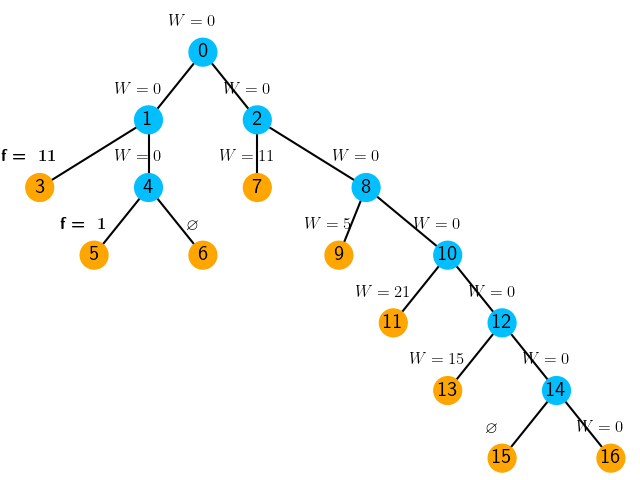
\includegraphics[scale=0.9]{branch_and_bound_tree.png}
  }
  \caption{Решение задачи методом ветвей и границ}\label{fig:part2_branch_and_bound_tree}
\end{figure}


На рисунке \cref{fig:part2_branch_and_bound_tree} представлено дерево решения задачи методом ветвей и границ. Каждый узел пронумерован согласно правилам \textit{\textbf{процедуры 1}}. Оранжевым цветом указаны листья, в которых либо получили расстановку станций, либо на данном множестве $G_\nu$ набор фиксированных и запрещенных переменных $\pi_{ij}$ делает недопустимым любое размещение (обозначено символом $\varnothing$).

Закрытие вершины осуществляется в случаях если:
\begin{enumerate}
  \item получен новый рекорд размещения;
  \item оценка <<недопокрытия>> больше рекорда, полученного на предыдущих итерациях;
  \item нет допустимого размещения БС.
\end{enumerate} 
Перейдем к исследованию множеств на возможность закрытия.

\textbf{Исследование множества $G_0$.}

За начальный рекорд примем длину всего отрезка $\widehat{P} = L = 50$.

Построение оценки $W(G_0)$:
$$
W(G_0)= \max\{L-2(r_1 + r_2), 0\} = \max\{50 -2(25+9), 0 \}.
$$

Разбиваем множества $G_0$ на два подмножества $G_1 = G^1_0$ ($\pi_{11} = 1$) и $G_2 = G^2_0$ ($\pi_{11} = 0$). Исследуем левое дочернее подмножество $G_1$. Правое подмножество $G_2$ оставим для обратного шага.

\textbf{Исследование множества $G_1$.}

Случай 1.

Проверка требования 1.

Шаг 1.

Проверяем, что каждый из радиусов $R_{10}$ и $R_{01}$ не меньше расстояния  до левого шлюза $s_0$. 
$$
l_1 - l_0 \leqslant R_{10} \rightarrow 20 - 0 \leqslant 62;
$$

$$
l_1 - l_0 \leqslant R_{01} \rightarrow 20 - 0 \leqslant 62;
$$

Шаг 2.
Осталось неразмещенная БС $s_2$. Проверяем, что радиусы связи $R_{12}$ и $R_{21}$ не меньше расстояния до правой точки от $a_1$ точка $a_2$.
$$
l_2 - l_1 \leqslant R_{12} \rightarrow 30 - 20 \leqslant 35;
$$

$$
l_2 - l_1 \leqslant R_{21} \rightarrow 30 - 20 \leqslant 28.
$$

Шаг 3.

Так как осталась только одна нераспределенная станция $s_2$, проверяем, что расстояние среди еще незанятых точек справа от точки $a_1$  есть такая точка, что расстояния от этой точки до точки $a_1$ и одновременно от этой точки до точки $a_{n+1}$ не больше, чем  радиус связи у нераспределенной станции.

Проверка точки $a_2$.
$$
l_2 - l_1 \leqslant R_{21} \rightarrow 30 - 20 \leqslant  28;
$$

$$
l_4 - l_2 \leqslant R_{21} \rightarrow 50 - 20 \leqslant  31;
$$

Проверка точки $a_2$.
$$
l_3 - l_1 \leqslant R_{21} \rightarrow 40 - 20 \leqslant  28;
$$

$$
l_4 - l_3 \leqslant R_{21} \rightarrow 50 - 40 \leqslant  31;
$$

Проверка обеспечения связи между размещаемыми БС произведена, можно приступать к оценке недопокрытия.

Случай 2.

Построение оценки $W(G_1)$:

$$
W(G_1) = w_1(G_1) + w_2(G_1).
$$

Недопокрытие слева от размещаемой БС $s_1$:

$$
w_1(G_1) = \max\{(l_1 - l_0) - r_1, 0\} \rightarrow \max\{(20 - 0) - 25, 0\} = 0.
$$

И оценка недопокрытия справа от размещаемой БС $s_1$: 
$$
w_2(G_1) = \max\{(l_4 - l_1) - (r_1 + 2r_2), 0\} \rightarrow \max\{(50 - 20) - (25 + 2 \cdot 9, 0\} = 0.
$$

Итоговая оценка
$$
W(G_1) = 0 + 0 = 0.
$$

Разбиваем множества $G_1$ на два подмножества $G_3 = G^1_1$ ($\pi_{22} = 1$) и $G_4 = G^2_1$ ($\pi_{22} = 0$). Исследуем  левое дочернее подмножество $G_3$. Правое подмножество $G_4$ оставим для обратного шага.

\textbf{Исследование множества $G_3$.}

Случай 1.

Проверка требования 1 проводится аналогичным образом. Перейдем к расчету оценки.

Случай 2.

Построение оценки $W(G_3)$:

$$
W(G_3) = w_1(G_3) + w_2(G_3).
$$

Недопокрытие слева от размещаемой БС $s_2$:

$$
w_1(G_3) =  w_1(G_1) + (l_2 - l_1) - (r_1 + r_2) \rightarrow 0 + \max\{(30 - 20) - (25+ 9), 0\} = 0 + 0 = 0
$$

Оценка недопокрытия справа от размещаемой БС $s_2$: 
$$
w_2(G_3) = \max\{(l_4 - l_2) - r_2, 0\} \rightarrow \max\{(50 - 30) - 9, 0\} = 11.
$$

$$
W(G_3) = 0 + 11 = 11.
$$

Все $m$ станции размещены, $f(P_1) = W(G_3)$. Так как $f(P_1) \leqslant f(\widehat{P}) \rightarrow f(P_1) \leqslant 50$, полученное недопокрытие $f(P_1)$ принимается за новый рекорд.

Следующим этапом будет обратный шаг по дереву поиска, так как все станции размещены, то есть нет свободных переменных $\pi_{ij}$ в множестве $\Pi^f$. Незакрытая вершина с наибольшим порядковым номером -- вершина $G_4$ с условием $\pi_{22}=0$.

\textbf{Исследование множества $G_4$.}


Случай 2.

Оценка правого дочернего узла $W(G_4)$ равна оценке материнского узла $W(G_1)$, $w_1(G_4)=w_1(G_1)$, $w_2(G_4) = w_2(G_1)$, и $W(G_4) = W(G_1) = 0$.


Разбиваем множества $G_4$ на два подмножества $G_5 = G^1_4$ ($\pi_{32} = 1$) и $G_6 = G^2_4$ ($\pi_{32} = 0$).

\textbf{Исследование множества $G_5$.}

Случай 1. Успешная проверка требования 1.


Случай 2.

Построение оценки $W(G_5)$:

$$
W(G_5) = w_1(G_5) + w_2(G_5).
$$

Недопокрытие слева от размещаемой БС $s_2$:

$$
w_1(G_5) =  w_1(G_5) + (l_3 - l_1) - (r_1 + r_2) \rightarrow 0 + \max\{(40 - 20) - (25+ 9), 0\} = 0 + 0 = 0
$$

Оценка недопокрытия справа от размещаемой БС $s_2$: 
$$
w_2(G_5) = \max\{(l_4 - l_3) - r_2, 0\} \rightarrow \max\{(50 - 40) - 9, 0\} = 1.
$$

$$
W(G_5) = 0 + 1 = 1.
$$

Все $m$ станции размещены, $f(P_2) = W(G_5)$. Так как $f(P_2) \leqslant f(\widehat{P})$, полученное недопокрытие $f(P_2)$ принимается за новый рекорд.


\begin{table}[h!]\centering
  \begin{tabular}{| c | c | c | c | c  c c|}
  
  \hline
  \multirow{3}{*}{№}& Номер & Оценка & Недопокрытие, &  \multicolumn{3}{c|}{Размещение} \\

  &узла & недопокрытия,& $f(P)$ & &	&	\\ \cline{5-7}
  &дерева, $\nu$ &$W(G_\nu)$& & $a_1$&	$a_2$&	$a_3$\\
  \hline
  1&0 &0&50 & --&	--&	--\\
  2&1 &0& & $s_1$ &	--&	--\\
  3&3 &11& Рекорд & $s_1$ &	$s_2$&	--\\
  4&4 &0&  & $s_1$ &	--&	-- \\
  5&5 &1& Рекорд & $s_1$ &	--&	$s_2$ \\
  6&6 & 0& $\varnothing$& $s_1$ &	--&	-- \\
  7&2 &0& & --&	--&	--\\
  8&7 &11& & $s_2$&	--&	--\\
  9&8 &0& & --&	--&	--\\
  10&9 &5& & --&	$s_1$&	--\\
  11&10 &0& & --&	--&	--\\
  12&11 &21& & --&	$s_2$&	--\\
  13&12 &0& & --&	--&	--\\
  14&13 &15& & --&	--&	$s_1$\\
  15&14 &0& & --&	--&	--\\
  16&15 &0& $\varnothing$& --&	--&	--\\
  17&16 &0& & --&	--&	--\\

  \hline
\end{tabular}\caption{Решение методом ветвей и границ}\label{part4:branch_and_bound_solution}
\end{table}

В ходе движения по дереву поиска исследования вершин происходило аналогичным образом как показано ранее. Оптимальным решением задачи стала расстановка $P_2$ c нелопокрытием $f(P_2) = 1$. В таблице \cref{part4:branch_and_bound_solution} представлены полученные оценки в ходе движения по дереву ветвлений.  Все вершины закрыты, количество пройденных узлов бинарного дерева поиска МВиГ составляет 16.


\textbf{Решение полным перебором.}

В качестве оценки алгоритма, чтобы не зависеть от мощности аппаратного и программного обеспечения, рассмотрим количество пройденных узлов. Для сравнения решим задачу полным перебором.

\begin{figure}[ht]
  \centerfloat{
      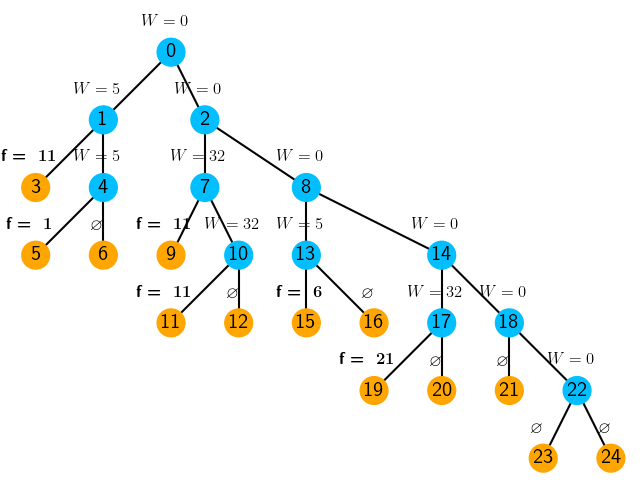
\includegraphics[scale=0.9]{brute_force_tree.png}
  }
  \caption{Решение задачи методом полного перебора}\label{fig:part2_brute_force_tree}
\end{figure}

Процесс решения задачи полным перебором представлен в виде бинарного дерева поиска на рисунке \cref{fig:part2_brute_force_tree}. В таблице \cref{part4:brute_force_solution} представлены полученные в ходе решения расстановки. Все расстановки пронумерованы в соответствии с порядком их нахождения. Оптимальным решением $P^*$ с минимальным значением функции \cref{eq:part3_P} является допустимая расстановка $P_2$. Количество пройденных узлов в ходе решения задачи составляет 24.

% \fontsize{10pt}{10pt}\selectfont
\begin{table}[h!]\centering
  \begin{tabular}{| c | c | c | c  c c|}
    \hline
    \multirow{2}{*}{Расстановка, $P$} & \multirow{2}{*}{Недопокрытие, $f(P)$} & \multirow{2}{*}{Номер узла дерева, $\nu$} &  \multicolumn{3}{c|}{Размещение} \\\cline{4-6}

    &&& $a_1$&	$a_2$&	$a_3$\\
    \hline
    $P_1$ & 11 & 3 & $S_1$ & $S_2$ & -- \\
    $P_2$ & 1 & 5 & $S_1$ & -- & $S_2$ \\
    $P_3$ & 11 & 9 & $S_2$ & $S_1$ & --  \\
    $P_4$ & 11 & 11 & $S_2$ & -- & $S_1$ \\
    $P_5$ & 6 & 15 & -- & $S_1$  & $S_2$\\
    $P_6$ & 21 & 19 & -- & $S_2$  & $S_1$\\
    \hline
    \multicolumn{3}{|c|}{Количество пройденных узлов} & \multicolumn{3}{|c|}{24} \\

    \hline
  \end{tabular}\caption{Решение полным перебором}\label{part4:brute_force_solution}
\end{table}

На примере частного случая размещения 2 БС по 3 точкам размещения было представлено МВиГ. Представлены деревья бинарного поиска для МВиГ и МПП. Предложенный метод позволяет сократить количество пройденный узлов в ходе поиска оптимального решения. 



% \fixme{==================================================}




\FloatBarrier
\section{Сравнения оценок «недопокрытия» для задачи 2, 3 и 4}\label{part4:task_234}

В таблице \cref{tab:part4_estimate_comparison} приведены результаты вычислительного эксперимента, показывающего время решения \underline{\textit{\textbf{задач 2, 3, 4}}} и относительную точность \underline{\textit{\textbf{задачи 3, 4}}} по отношению к \underline{\textit{\textbf{задаче 2}}}.

Для непокрытого участка справа длины $|\beta| = 50$, варьируя количеством не размещенных БС, а также количеством свободных мест размещения требуется рассчитать оценку недопокрытия при бюджетном ограничении $C=600$.


Как видно из результатов расчетов в таблице \cref{tab:part4_estimate_comparison}, представляется целесообразным  использовать  \underline{\textit{\textbf{задачу 4}}} в качестве оценки $w_2 (G_\nu )$ для решения задач большой размерности, так как время ее расчета в виде задачи ЛП существенно ниже с учетом высокой точности относительно \underline{\textit{\textbf{задачи 2}}}.


% \fontsize{8pt}{8pt}\selectfont
\begin{table}[h!]\centering
  \begin{tabular}{| c  | c  | c | c | c | c | c | c |c | c |}
    
    \hline
    \multirow{3}{*}{\rotatebox{270}{\thead{Количество точек \\ размещения, $m$}}}
    & \multirow{3}{*}{\rotatebox{270}{\thead{Количество  свободных\\ станций,  $|S_\beta|$}}}

    & \multicolumn{2}{|c|}{ЦЛП} 
    & \multicolumn{3}{|c|}{\thead{Задача \\
   <<О ранце>>}} 
    & \multicolumn{3}{|c|}{ЛП} \\\cline{3-10}

    && \multicolumn{2}{|c|}{Задача 2} 
    & \multicolumn{3}{|c|}{Задача 3} 
    & \multicolumn{3}{|c|}{Задача 4} \\\cline{3-10}

    &&\rotatebox{270}{Время расчета, сек } 
    &\rotatebox{270}{Недопокрытие, $z$}
    &\rotatebox{270}{Время расчета, сек} 
    &\rotatebox{270}{Недопокрытие, $z$}
    &\rotatebox{270}{Точность, \%}
    &\rotatebox{270}{Время расчета, сек} 
    &\rotatebox{270}{Недопокрытие, $z$}
    &\rotatebox{270}{Точность, \%}\\

    \hline
    5&	6&	0,3250&	436&	0,3214&	426,00&	97,71&	0,0047&	436,00&	100,00 \\
    5&	8&	0,3218&	431&	0,3582&	398,00&	92,34&	0,0045&	431,00&	100,00 \\
    8&	10&	0,3765&	395&	0,3621&	375,00&	94,94&	0,0094&	395,00&	100,00 \\
    8&	12&	0,3746&	390&	0,2977&	347,00&	88,97&	0,0094&	390,00&	100,00 \\
    12&	15&	0,3363&	339&	0,2960&	309,00&	91,15&	0,0114&	339,00&	100,00 \\
    12&	17&	0,4072&	336&	0,3456&	283,00&	84,23&	0,0136&	336,00&	100,00 \\
    18&	20&	0,3558&	265&	0,3407&	265,00&	100,00&	0,0121&	265,00&	100,00 \\
    18&	25&	0,3794&	260&	0,3096&	259,00&	99,62&  0,0169&	257,60&	99,08 \\
    25&	30&	0,3177&	246&	0,3576&	246,00&	100,00&	0,0222&	244,33&	99,32 \\
    25&	45&	0,3539&	229&	0,3556&	229,00&	100,00&	0,0494&	226,40&	98,86 \\
    30&	50&	0,2994&	225&	0.3146&	225,00&	100,00&	0,0570&	224,13&	99,61 \\
    30&	100& 0,5179& 223& 0,5177& 223,00& 100,00& 0,1513& 218,75& 98,09 \\
    \hline
  \end{tabular}\caption{Сравнение методо расчета оценок недопокрытия справа}\label{tab:part4_estimate_comparison}
  \end{table}
\normalsize




\section{Сравнительная оценка полученных модели ЦЛП и модели в комбинаторной форме, решаемой с помощью МВиГ}
Для решения задачи оптимального размещения базовых станций вдоль линейной территории были представлены математическая модель целочисленного линейного программирования и комбинаторная модель в экстремальной форме, для которой представлен специальный алгоритм на основе метода ветвей и границ, учитывающий специфику задачи -- размещение вдоль линейной территории и обеспечения связи между всеми размещенными станциями.

В обеих моделей предполагается, что из заданного множества БС может быть размещено любое количество станций, удовлетворяющих условиям задачи. Через систему размещенных БС необходимо обеспечить связь между левым и правым шлюзом. Для задачи ЦЛП размещение должно удовлетворять бюджетному ограничению. И для задачи в комбинаторной форме задача должна удовлетворять бюджетному ограничению и ограничению на величину межконцевой задержки сети.

Для того чтобы сравнить полученные модели, рассмотрим частный случай задачи максимизации покрытия с размещением всех имеющихся БС. Опустим бюджетное ограничение для обеих задач и для комбинаторной модели также ограничение на время задержки в сети. Вместо данных ограничений, добавим условие размещения всех имеющихся $m$ станций. Такая постановка позволит зафиксировать множество вариантов размещения, необязательно только допустимых. Общее количество $\gamma$ вариантов расстановки $m$ станций по $n$ точкам размещения выражается с помощью уравнения \cref{eq:part4_gamma}.


Для обеспечения условия размещения всех $m$ станций в случае комбинаторной модели представлено уравнение \cref{eq:part4_noncoverage_estimation2}. Для задачи ЦЛП данное условие будет выглядеть следующим образом:


\begin{equation}
  \label{eq:part3_placed_all_station}
  \sum\limits_{i=1}^n \sum\limits_{j=1}^m x_{ij} = m.
\end{equation}

Для различных случаев числа мест размещения $m$ и числа станций $n$ сравним результаты решения задачи представленными моделями. Оценка сравнения с помощью времени счета необъективна, так как предложенный алгоритм МВиГ и сама комбинаторная модель написаны на интерпретируемом языке Python. Коммерческие продукты представляют быстрые и качественные инструменты. Написание производительного кода для предложенных в данной диссертации моделей является отдельной не простой задачей, выходящей за рамки данного исследования. Коммерческие продукты решающие задачи ЦЛП основаны на алгоритме, предложенном Алисой Лэнд и Элисон Дойг \cite{Land1960}, в котором процедура поиска целочисленного решения также использует МВиГ.  Поэтому для сравнения моделей будет использована характеристика -- число просмотренных вершин в ходе поиска оптимального решения. Для сравнения также будут представлены решения задачи в комбинаторной форме методом полного перебора (МПП).

Для каждого набора станций и мест размещения было рассчитано по 10 примеров с различными параметрами БС. В таблице \cref{tab:models_comparation} приводятся усредненные показатели числа просмотренных вершин дерева поиска по каждым 10 примерам. Результаты решения задачи максимизации покрытия влияют не только от количества точек размещения $n$, но также от их координат. Примем, что для каждой размерности для всех 10 примеров координаты фиксированы для всех моделей: МПП, МВиГ и ЦЛП. 


\begin{table}
  \caption{Результаты численного решения.}\label{tab:models_comparation}
  \begin{tabular}{|ccc|*{3}{c}|} \cline{3-6}
  \hline
  \textbf{Число точек} & \textbf{Число} &\textbf{Количество} & \multicolumn{3}{c|}{\textbf{Количество пройденных}}\\ 
  \textbf{размещения,} & \textbf{cтанций,} & \textbf{вариантов} & \multicolumn{3}{c|}{\textbf{узлов дерева поиска, $\nu$}}\\
  \cline{4-6}
  \textbf{$n$} & \textbf{$m$} &\textbf{размещения, $\gamma$} & \textbf{МПП}& \textbf{МВиГ} & \textbf{ЦЛП} \\ 
  \hline
  7 &  4 & 840 & 3122 & 360 &  \textbf{275} \\
  7 &  5 & 2 520 & 16 114 & 560  &  \textbf{45}  \\
  7 &  6 & 5 040 & 59 564 & 364  &  \textbf{19}  \\
  8 &  4 & 1 680 &  4954 &  434 &   \textbf{189} \\
  8 &  5 & 6 720 & 6720 & \textbf{852}  &  878 \\
  8 &  6 & 20 160 &  15 9170 & 592  & \textbf{185}  \\
  9  &  4 & 3 024 & 9 882 & \textbf{458} & 5511 \\
  9  &  5 & 15 120&  58 190 &  \textbf{768} &  1236\\
  9  &  6 & 60 480&  366 512 &  \textbf{720} & 13294 \\
  10 &  4 & 5 040&  14 868&  \textbf{800}&  6243\\
  10 &	5 & 30 240&  113 932&  \textbf{414}&  8043\\
  10 &	6 & 151 200&  828 952&  \textbf{40 872}&  71587\\
  11 &  4 & 7 920& 23 482&  \textbf{354} & 15538\\
  11 &	5 & 55 440& 204 894& \textbf{9 138}&  74440\\
  11 &	6 & 332 640& 1 592 500 & \textbf{88 002} & 413 767 \\
  \hline
  \end{tabular}
\end{table} 
\normalsize

Жирным цветом в колонках пройденных узлов в ходе движения по дереву поиска МПП, МВиГ и ЦЛП выделены минимальные значения для фиксированных значений $n$ и $m$ (размерностей задачи). Как видно из результатов сравнения, при увеличении размерности задачи разработанный алгоритм метода ветвей и границ для комбинаторной модели показывает лучшие результаты по сравнению с математической моделью ЦЛП.
% \FloatBarrier
\section{Выводы по главе 4}

\begin{enumerate}
  \item Представлен программный комплекс для расчета задачи оптимального размещения базовых станций
  \item Рассмотрен численный пример оптимального размещения БС в виде задачи ЦЛП;
  \item Рассмотрен численный пример оптимального размещения БС задачи  в виде комбинаторной модели в экстремальной форме;
  \item Рассмотрен пример процедура нахождения последовательности лучших решений с помощью предложенного МВиГ;
  \item Представлен поиск оптимального размещения с помощью предложенного МВиГ на примере размещения двух станций;
  \item Представлено сравнение методов оценки недопокрытия справа;
  \item Представлена сравнительная оценка полученных модели ЦЛП и модели в комбинаторной форме, решаемой с помощью МВиГ.
\end{enumerate}
